\clearpage
\section*{LAMPIRAN}
\phantomsection
\addcontentsline{toc}{section}{LAMPIRAN}

% 1. Reset penomoran gambar agar dimulai dari L.1, L.2, dst.
\setcounter{figure}{0} 
\renewcommand{\thefigure}{L.\arabic{figure}}

% 2. Pastikan label yang muncul adalah "Gambar", bukan "Figure"
\renewcommand{\figurename}{Gambar}

\vspace{1cm}
\noindent
\textbf{HASIL PENGUJIAN UNIT (UNIT TESTING)}

\noindent
Lampiran ini menyajikan data teknis hasil audit pengujian unit yang dilakukan terhadap seluruh fungsionalitas backend Sistem POS WellClean Laundry menggunakan tool \texttt{go tool cover}. Pengujian ini memvalidasi integritas logika baris kode pada setiap fungsi utama.

\begin{figure}[H]
    \centering
    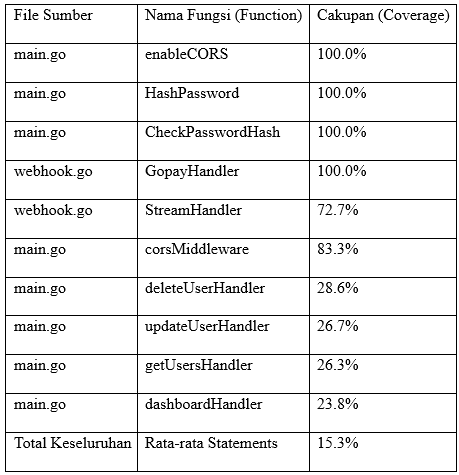
\includegraphics[width=0.8\textwidth]{images/rekapitulasi.png}
    \caption{Rekapitulasi Cakupan Baris Kode (Statements)}
    \label{fig:rekapitulasi}
\end{figure}

\begin{figure}[H]
    \centering
    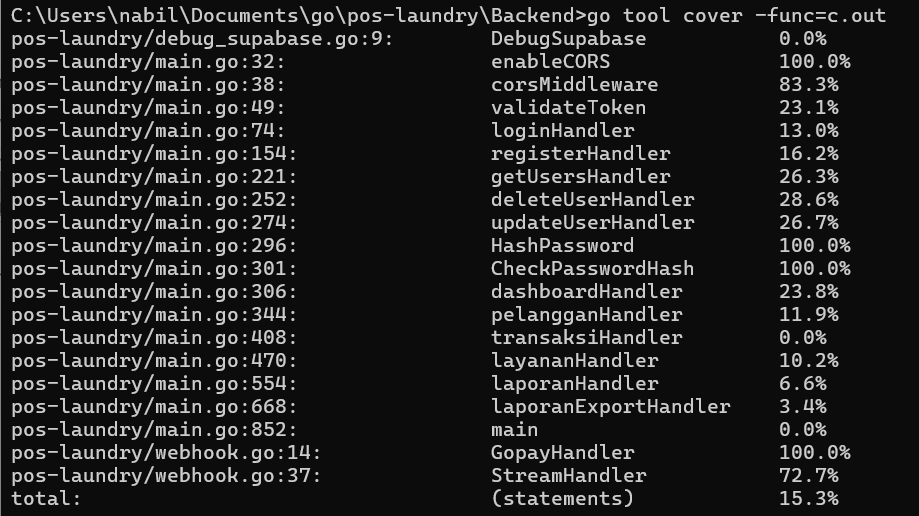
\includegraphics[width=0.8\textwidth]{images/codecoverage.png}
    \caption{Tangkapan Layar Hasil Codecoverage}
    \label{fig:codecoverage}
\end{figure}